\section{Theorem D and the ring of contingency tables}\label{sec:ehrhart}
The companion \cite{CouplingAlgebras} puts the geometry of couplings into a graded ring: the Ehrhart ring of a polytope of tables with
rational margins. Its degree-$k$ piece has the integer tables with $k$ times the margins as a basis. Its Hilbert function counts them,
and the count crosses the walls of the margin space by one binomial term at a time. A reviewer asked two questions about it. Is the
decision functional of \cref{thm:D}, the worst case of an act over the hiding set, a section of this ring? And is the settling size
$n^*$ a wall-crossing? The short answers are no and no. The ring does give two things, though: the correct algebraic form of the worst
case, and an exact probe that settles sooner. This section works it out for three binary variables, the case of \cref{thm:D}(4).

\paragraph{The fibre.} Fix the three pair tables of a law $P$ on $\{0,1\}^3$. The laws that share them form a segment
$P+\varepsilon\chi$, with $\chi(x)=\prod_i(2x_i-1)$. This is the no-three-way-interaction model. Its toric ideal is principal, generated by
the single quartic $p_{000}p_{011}p_{101}p_{110}-p_{001}p_{010}p_{100}p_{111}$ (Macaulay2, check EH1), so $\chi$ is its only Markov
move. Moving along the fibre moves the triple moment at unit speed, because
\[
m_T(P+\varepsilon\chi)-m_T(P)=\varepsilon\sum_x\chi(x)\prod_i(x_i-\mu_i)=\varepsilon\prod_i\bigl((1-\mu_i)+\mu_i\bigr)=\varepsilon .
\]
So the fibre is an interval of $m_T$, ended where a cell reaches zero. If $P$ has denominator $N$, then at sample size $n=kN$ the integer
tables with the pair tables of $nP$ are the points $nP+j\chi$, $j\in\mathbb Z$, a lattice of step $1/n$ in $m_T$. The hiding set $R$
of \cref{thm:A} is the part of this interval where a two-type explanation exists, $m_T\in v_T\,[r_-,r_+]$.

\begin{proposition}[the hiding set inside the ring]\label{prop:ehrhart}
For three binary variables and a two-type law $P$ with denominator $N$:
\begin{enumerate}
\item[(i)] The integer tables with the pair tables of $kNP$ are the lattice points of $k$ times a lattice segment of length $\ell$. Their
number is the Ehrhart polynomial $k\ell+1$, the degree-$k$ Hilbert function of the ring.
\item[(ii)] $R$ is a strict sub-segment. Its ends are where some $a_{ji}$ reaches $0$ or $1$, while every cell of the law is still
positive. Those ends are algebraic numbers and generally irrational. So the number of tables in $kR$ is not an Ehrhart polynomial, and
not even a quasi-polynomial.
\item[(iii)] The expected utility of an act on the three variables is affine on the fibre, $U_a=U_a(P)+c_a\,(m_T-m_T(P))$. Its slope is
the Walsh coefficient $c_a=\sum_xu_a(x)\chi(x)$, and $\beta_a=v_Tc_a$ in the coordinate $r$.
\end{enumerate}
\end{proposition}

\begin{proof}
(i) Every cell of a table with the given pair tables is an integer plus or minus one free integer, so the fibre is $T_0+\mathbb Z\chi$,
cut by $T_0+j\chi\ge0$. The ends are integers, and dilating by $k$ multiplies them by $k$. (ii) The ends of $R$ are the ends of
\cref{thm:A}'s box, where a coordinate of $a_1=\mu+vt$ or $a_2=\mu-v/t$ reaches $0$ or $1$; a cell of the mixture vanishes only if both
components vanish there. The count is $\lfloor n\,(R_+-m_0)\rfloor-\lceil n\,(R_--m_0)\rceil+1$. With irrational ends, its second
differences at any fixed period do not vanish. (iii) This is the computation above with $u_a$ in place of the moment.
\end{proof}

For the worked truth $w=\tfrac25$, $a_1=(\tfrac45,\tfrac3{10},\tfrac7{10})$, $a_2=(\tfrac15,\tfrac7{10},\tfrac3{20})$, the denominator is
$N=5000$. The fibre is $m_T\in[-0.0671,\,0.0609]$, a lattice segment of 640 steps. The hiding set $R=[-0.0214,\,0.0100]$ is $25\%$ of
it (\cref{fig:ehrhart}(a)).

\begin{proposition}[the decision functional and the ring]\label{prop:tropical}
\begin{enumerate}
\item[(i)] \emph{Not a section, but a tropical limit.} The worst value $W_a$ is a minimum of linear forms, so it is not an element of the
ring. It is the limit of a weighted count over the same basis of tables:
\[
\min_{T}U_a(T)-\frac{\log\#}{s}\ \le\ -\frac1s\log\sum_{T}e^{-sU_a(T)}\ \le\ \min_{T}U_a(T),
\]
where $T$ runs over the tables in $nR$ (or in the whole fibre) and $\#$ is their number. As $s\to\infty$ the middle term tends to the
lattice minimum. That minimum is $W_a$ exactly over the fibre, whose ends are lattice points, and within $|c_a|/n$ over $R$.
\item[(ii)] \emph{Over the whole fibre the worst case is an integer programme.} Take the quartic, oriented so that its leading term is
the costlier side. Its normal form (Conti--Traverso) is the table that minimises $U_a$. As a function of the pair tables this minimum is
piecewise linear. It breaks only where the binding cell changes, and those are the walls where the fibre's length, the leading
coefficient of the table count, breaks too. So a skeptic who allows every law with the given pair tables has decision walls that are
linear on each chamber of \cite{CouplingAlgebras}. The set rule on $R$ has algebraic walls instead, because positivity of the
explanation, not of the table, ends $R$.
\item[(iii)] \emph{$n^*$ is not a wall-crossing.} Raising $n$ moves the margins along a ray, and chambers are cones. So the table count
stays one polynomial, and no wall is crossed. The lattice is still visible at $n^*$, though. The truth sits
$n^*d\,|v_T|=(z\tau)^2|v_T|/d$ lattice steps from the decision wall: about ten in Study 11b's designs. The conditional law of the
position has standard deviation $\tau_c|v_T|\sqrt{n^*}$, about five steps.
\item[(iv)] \emph{The exact probe is the efficient one.} Given its own pair tables, the triple window is a lattice point on its fibre.
Its conditional law is the exponential family $\propto e^{\psi j}/\prod_x(T+j\chi)_x!$ in the three-way log odds ratio
$\psi=\sum_x\chi(x)\log p_x$. This is the sample space of Fisher's exact test in \cite[Thm.~7.1(iv)]{CouplingAlgebras}, tilted. Mapping
$\psi$ to $r$ through the known pair tables gives an estimate with asymptotic standard deviation
\[
\tau_c=\frac{1}{|v_T|\sqrt{\sum_x1/p_x}}\ \le\ \tau_m ,
\]
where $\tau_m$ is that of the plug-in moment (with $v$ known). The inequality is Cram\'er--Rao along the fibre, because $\sum_x1/p_x$ is
the Fisher information of the move. So with the pair tables known, the exact probe settles at the smaller size $n^*_c=(z\tau_c/d)^2$.
\end{enumerate}
\end{proposition}

\begin{proof}
(i) Bound the sum between its largest term and $\#$ times its largest term. Over the fibre the minimum of an affine function is at an
end, and the ends are lattice points (\cref{prop:ehrhart}(i)). Over $R$ the nearest lattice point to an end is within $1/n$ of it.
(ii) The Gr\"obner basis of a principal ideal is its generator, and reduction by it applies the move against the cost while the table
stays nonnegative. The end it reaches is $\min_x$ of a linear form in the margins, taken over the cells with the right sign of $\chi$;
both this minimum and the fibre's length change formula exactly where the argmin changes. (iii) A ray $kNP$ has fixed binding cells
(check EH5). At $n^*$ the post-probe half-width $z\tau/\sqrt{n^*}$ equals $d$; in lattice steps that is $n^*d|v_T|$. (iv) The
conditional law is classical, with sufficient statistic $j$. The Fisher information of $P+\varepsilon\chi$ in $\varepsilon$ is
$\sum_x\chi(x)^2/p_x$. The plug-in moment is a regular estimator of $\varepsilon$ on this one-parameter model, so its variance is at least
the inverse information.
\end{proof}

Checks EH1--EH7 (\texttt{engine/check\_ehrhart.py}) verify each statement, as follows.
\begin{itemize}
\item EH1: the brute-force counts.
\item EH2: the quasi-polynomial test, for periods up to $12$.
\item EH3: the tropical bounds, on three acts.
\item EH4: Conti--Traverso against enumeration and linear programming, and the kinks along lines of margins.
\item EH5: the lattice reading of $n^*$.
\item EH6: $\tau_c\le\tau_m$ on 300 random truths, and a simulation of the conditional MLE.
\item EH7: the exactness of the conditional interval, coverage at least $0.95$ at every $\psi$.
\end{itemize}

\subsection*{Study 11c: settling with the exact conditional probe}
Proposition~\ref{prop:tropical}(iv) makes a prediction that can fail. A regulator who knows the pair tables and uses the exact
conditional interval for $\psi$ should settle at $n^*_c$, earlier than the plug-in regulator of Study 11b. But exact intervals are
conservative, and at $n^*$ the conditional law spans only a few lattice steps. Study 11c was registered and frozen with SHA-256 before
any registered design was simulated (\texttt{engine/study11c\_exact/PREREG\_study11c.md}), after the checks above and one smoke run on an
invented design. It reuses Study 11b's designs D2, D3, D5 and the stratum D4, with the pair tables known. One triple window feeds both
probes, and there are 2000 replicates per cell.

\begin{table}[!htbp]\centering\small
\begin{tabular}{p{0.06\linewidth}p{0.56\linewidth}p{0.30\linewidth}}\toprule
& prediction & outcome\\\midrule
E1 & exact probe's median settling size within a factor $1.25$ of $n^*_c=(z\tau_c/d)^2$ & holds: ratios $1.08$, $1.06$, $1.09$\\
E2 & exact probe's median below the plug-in probe's in every design & \textbf{fails}: D2 $2735<2799$, D3 $5285<5612$, but D5 $1954>1860$\\
E3 & exact settling rate within $0.06$ of the normal theory with $\tau_c$ at every $n$ & holds: largest gap $0.046$\\
E4 & D4 (stratum): exact rates at $n=3000$ and $10^5$ within $0.05$, both below one half & holds: $0.021$ and $0.020$ (plateau $0.025$)\\\bottomrule
\end{tabular}
\caption{Study 11c: registered predictions and outcomes.}\label{tab:study11c}
\end{table}

Three of the four predictions held, and one failed (\cref{tab:study11c}, \cref{fig:ehrhart}(d)). The exact probe settles close to
$n^*_c$, but always a little later. Its medians are $6$--$9\%$ above $n^*_c$, and its rate sits below the normal-theory curve at every
$n$ up to $4n^*_c$. This is the price of an exact interval: its coverage is at least $95\%$, never exactly $95\%$ (check EH7), and at
$n^*$ only a few lattice steps carry the conditional law.

E2 failed in one design. The efficiency gain is $(\tau_m/\tau_c)^2$ in sample size. That is $12\%$ for truth G, which beats the
conservativeness, so in D2 and D3 the exact probe settled first. For truth H the gain is $8\%$, and conservativeness ate it: in D5 the
exact probe settled $5\%$ later than the plug-in. So the exact probe is the efficient one in the limit, but not uniformly better at
$n^*$. A mid-$p$ interval, which is less conservative, is the natural repair. It was not registered, and it is not tested here.

On the stratum D4 neither probe settles. With the pair tables known, the plateau is the one-sided $2.5\%$ of \cref{thm:D}(4c), not
Study 11b's $0.27$. That larger value came from the noise in the estimated pair tables.

\begin{figure}[!htbp]\centering
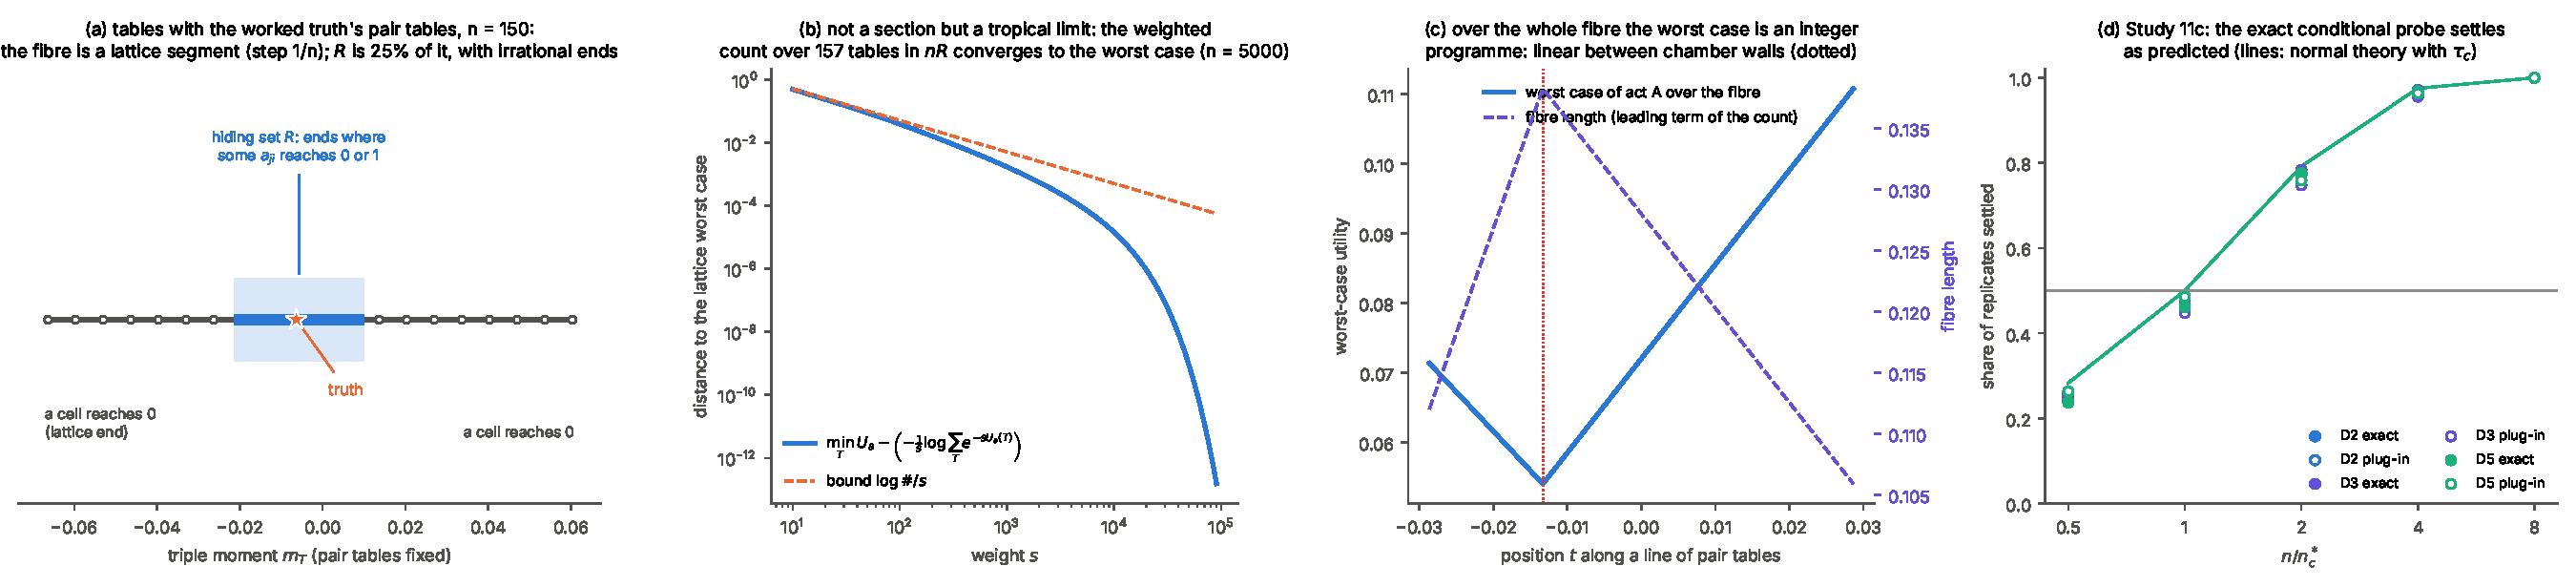
\includegraphics[width=\linewidth]{fig_ehrhart.pdf}
\caption{The decision and the ring of contingency tables. (a) The worked truth. The tables with its pair tables form a lattice segment
in $m_T$, shown at $n=150$ (dots). The hiding set $R$ (blue) is a quarter of it, ended by the explanation's positivity walls rather than
by a table's. (b) Act A's worst case over the tables in $nR$ as a tropical limit. The distance from the weighted count to the
lattice minimum stays below $\log\#/s$ and vanishes as $s$ grows. (c) Over the whole fibre, the worst case along a line of pair tables is linear between chamber walls
(dotted), where the fibre's length (dashed) also breaks. (d) Study 11c: settling with the exact conditional probe (filled) and the
plug-in probe (open) against $n/n^*_c$; the lines are the normal theory with $\tau_c$.}\label{fig:ehrhart}
\end{figure}

\paragraph{Gap 3, answered.}
\begin{itemize}
\item \emph{Is the decision functional a section?} No. The worst case is a tropical object: the $s\to\infty$ limit of a weighted Hilbert
  function. Over the whole margin fibre it is an integer programme solved by the toric ideal's Gr\"obner basis, and linear on chambers.
  Over the hiding set it is not polyhedral, because positivity of the explanation, not of the table, draws its walls.
\item \emph{Is $n^*$ a wall-crossing?} No. Raising $n$ moves along a ray inside one chamber. What does cross a wall is the truth leaving
  the stratum $d=0$, and that is a change of design, not of sample size.
\item \emph{What the ring contributes.} The ring supplies the exact sample space of the probe. Using it is the efficient way to settle,
  $\tau_c\le\tau_m$, and Study 11c measures what conservativeness costs at the few lattice steps that matter at $n^*$.
\end{itemize}
